\section{Inteligência Artificial}

Inteligência é, por definição, uma coleção sistemática de habilidades e funções com objetivo de processar diferentes tipos de informações de diversas maneiras \cite[49]{guilford1982cognitive}. Simular essa "coleção sistemática de habilidades e funções", reconhecer formatos, trajetórias, sinais, deduzir proposições entre outras, criando entidades inteligentes é o foco da inteligência artificial.

Do momento em que a IA passou a ser um campo de estudo em 1950, com as propostas de Turing, até o momento atual, a quantidade de abordagens apresentadas por diversos pesquisadores, afim de construir uma máquina inteligente apenas aumentou. Esses métodos se auto-contribuíram propondo novas visões e gerando novas abordagens a partir de descobertas dentro das suas linhas de pensamento. Isso levou a IA para seu estado atual. \cite[1-2]{russell2003artificial}.

No decorrer desta sessão serão apresentados os fundamentos visando introduzir as demais áreas que colaborarão com a computação para a criação da inteligência artificial, seguido pelas definições de agentes racionais.

\subsection{Fundamentos da Inteligencia Artificial}
Nas últimas sessões foram abordados os temas linguística e psicologia, e claramente é possível vislumbrar sua relevância dentro da área de Inteligência Artificial. A razão é o fato de ambas serem fundamentos da IA assim como outras áreas que serão dissertadas nessa sessão.

A engenharia da computação tem como foco construir máquinas eficientes, seja impactando com novos \textit{hardwares}, afetando diretamente o potencial de processamento e armazenamento das máquinas, ou com a criação de novos sistemas operacionais, linguagens e ferramentas que podem desde auxiliar na \textit{performance}, organização ou complexidade do problema até possibilitar criação de novas abordagens e implementações de algoritmos mais complexos. \cite[13-14]{russell2003artificial}.

Na busca de um melhor resultado durante a criação de um sistema inteligente, o processamento de dados é algo essencial. Em certos momentos os dados não fornecerão diretamente o que é necessário, e o ato de assimilar uma verdade baseado em outra verdade já conhecida, também chamado de inferência, já não será suficiente para gerar bons resultados, sendo assim, é necessário utilizar de recursos fundamentados e probabilísticos como equações matemáticas para resolver o problema. Para que isso se torne possível, será necessário extrair um dado exato de algo abstrato, por exemplo o \textit{sentistrength}, que retira o sentimento a partir de um trecho de texto \cite{boole1854investigation}.

Além dos conceitos de matemática, existem fatores da economia que fundamentam a IA. Diferente do que sugerido, essa área não se trata de dinheiro, mas de como é guiada as decisões baseadas nos retornos esperados. Os estudos da economia ainda aplicam-se a como agir perante expectativas de curto, médio ou longo prazo e se é viável continua-las quando outros fatores não estiverem favorecendo o ambiente \cite[9]{russell2003artificial}. Abordando o ambiente não só como o \textit{software} e sim como um mundo externo a ele, existe um fundamento, que não será aprofundado por não ter impacto nesta pesquisa, nomeado cibernética e a teoria de controle. Foi criado por Wiener\cite{wiener1961cybernetics} e visa o uso de componentes elétricos para coletar informações externas á máquina e traduzi-los para uma linguagem (numérica) na qual a máquina seja capaz de compreender.

Existem campos, como a própria linguística citada, que procuram sair da forma descritiva que atuam, propondo-se adotar modelos e definições exatas para guiar seus estudos. Esse foi o caso da neurociência, que é responsável por estudar o cérebro humano, ou seja, como as redes neurais funcionam \cite[10]{russell2003artificial}.

A biologia em si era em grande parte descritiva, embasada por anos de observação e pesquisas que até hoje apoiam suas definições. Sair desses padrões levou os cientistas a vislumbrarem a possibilidade de tratar o metabolismo como um centro de transmissão. Esse centro enviaria diversas transmissões que por sua vez emitiriam uma força. Essa afirmação levaria os cientistas a poderem calcular a força dessas transmissões afim de chegar em um modelo matemático plausível para replicar o funcionamento das redes neurais \cite[1-3]{rashevsky1960mathematical}. Entretanto, duvidas como até onde pode-se um computador suportar ou superar o processamento de um cérebro humano foram levantadas. Mesmo com tantas discussões em torno do assunto, a proposta de Vinge sobre uma super-máquina que superaria a inteligência humana, também chamada de singularidade tecnológica, continua não tendo uma comparação informativa atualmente, e mesmo que atualmente existisse a capacidade de ter-se memória e processamento infinito ainda não é possível entender como armazenar e replicar os padrões encontrados na neurociência \cite[11-12]{vinge1993coming,russell2003artificial}. Os estudos cognitivos tornaram possível entender melhor o funcionamento da mente humana. O método racional e a proposta de pensar nos meios que nos levam a um fim fez com que fosse capaz de abstrair modelos inteligentes através de agentes. A neurociência, por sua vez, forneceu a magnitude de como transmitir conhecimento e aprimorar os modelos, o fator inteligência e aprendizado passaram a ser mais vistos dentro do ramo de IA, nos levando a ascensão da aprendizagem de máquina.

Diferente das ciências onde existem fatos, teorias e pesquisas conclusivas, existem áreas capazes de fomentar intelectualmente assuntos diversos. O conceito de lógica, por exemplo, é algo relativamente descritível e aplicável aos conceitos da ciência, porém a teoria por trás do que viria ser lógico e o que faria um pensamento ser racional é algo muito mais complexo, em suma, o conceito de lógica já era debatido por estudiosos na Grécia antiga. A filosofia tem sua relevância pra IA pois contribuiu com ideias como o \textit{Law of thought} (lei do pensamento), que em contra partida ao pensar humano, é uma lei psicológica que acompanha um processo mental, logo, necessita estar de acordo com uma razão ou lógica \cite{frege1956thought, russell2003artificial}. Além disso, a filosofia foi responsável por estudos como o racionalismo onde é dito que é possível adquirir conhecimento independente da experiência sensorial. Originada dessa ideia nasceram o dualismo, onde é afirmado que a mente é algo natural e sem conhecimento do mundo externo, e o materialismo, que contrariando o dualismo afirma que a mente é formada pelas operações do cérebro. Em negativa ao racionalismo, existe o empirismo, onde é definido que a experiência sensorial é a fonte final de conhecimento \cite[6]{rationalismvsempiricism, descartes2013rene, russell2003artificial}. Estes estudos tiveram sua relevância sobre o pensamento racional e como seria possível criar máquinas que pensassem e agissem racionalmente.

\subsection{Agentes Racionais}
“Mas seria possível uma máquina pensar?“ Esse questionamento inicial de Turing, desencadeou a proposta do \textit{Imitation Game}, que basicamente consiste em colocar uma pessoa (1) para conversar com um computador, esse computador poderá ser uma inteligência artificial ou outra pessoa (2) conversando através da máquina. O objetivo é que a pessoa 1 consiga distinguir se quem esta conversando com ela é a máquina ou a pessoa 2. A proposta feita por Turing seria considerada como um agir humanamente. Ela baseia-se em criar uma máquina que reconhece a escrita, tome decisões a partir de um base de dados e por final seja capaz de se aprimorar diante de novos cenários. Porém, como seria desenvolvido algo de tal amplitude? A resposta é que “não seria”! Questionar se uma máquina é capaz de pensar seria o mesmo que questionar se um submarino é capaz de nadar, afirmou Dijsktra, apontando que o termo "pensar" e "nadar" tinham suas definições restritas, entretanto, era possível realizar ações similares tão bem quanto \cite[2-3]{dijkstra898, turing1950, russell2003artificial}.

Para realizar as ações descritas por Turing, é necessário entender os passos descritos por ele de forma racional e lógica afim de replicá-los para a máquina.

A abordagem de agentes racionais é uma das possibilidades a serem usadas. O termo racional significa algo baseado ou acordado com uma razão ou lógica, de outro lado, a lógica tem dois pilares: a conversão responsável por expressar a mesma proposição em diferentes formas e o silogismo responsável por localizar um termo em comum que conecte duas dessas proposições. Um agente é algo que age, ou seja, um agente racional seria quem analisa circustâncias utilizando de definições lógicas e racionais a fim de interagir com algo. Isso é afirmado pela definiçao de Russel\cite[7]{russell2003artificial}, onde um agente racional percebe modificações no ambiente, através de sensores, e interage de volta com o ele novamente através de atuadores. Pode-se notar esse fluxo na Figura \ref{fig:rational_agent_draw}.

Logo, é possivel afirmar, que para ser possível realizar ações racionais é necessário entender o ambiente aonde você esta e suas variáveis, alias, é necessário que esteja claro o que pode ou não ser computado, quais são as regras que se aplicam e principalmente como obter algo racional com base em informações abstratas ou com dados incompletos \cite{frege1956thought, wooldridge1994agent, simon1955behavioral, boole1854investigation, russell2003artificial}

\begin{figure}
    \centering
    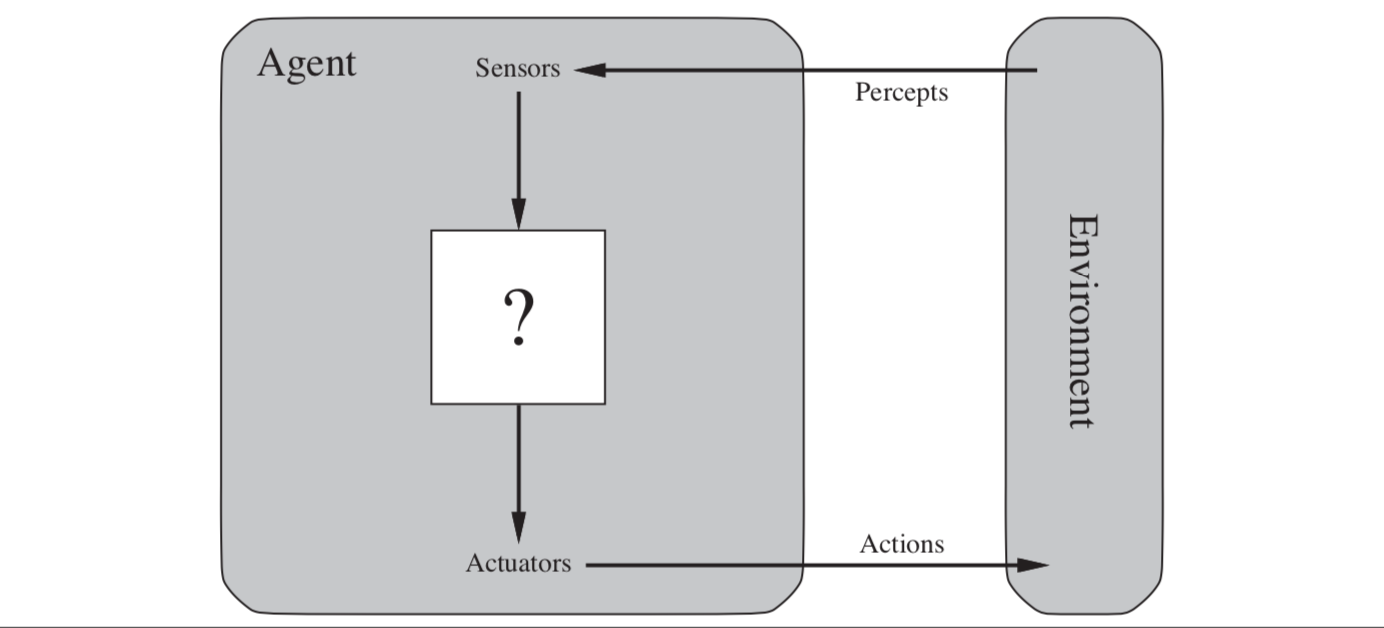
\includegraphics[width=.8\textwidth]{imagens/rational_agent_draw.png}
    \caption{Fluxo executado por um agente racional. Fonte: Russel, 2003, 35. Adaptada pelo Autor}
    \label{fig:rational_agent_draw}
\end{figure}

Definir se o agente está ou não gerando os dados esperados é um dos passos durante o desenvolvimento dos agentes. É necessário analisar o ambiente gerado a partir das percepções e conferir se os dados são os esperados ou não, essa etapa chama-se mensuração de \textit{performance}. Resumidamente, o agente receberá um entrada de dados e será responsável por gerar um saída. Ao longo do tempo o mesmo agente gerara múltiplas percepções e essas formarão uma sequencia de percepções \footnote{Não serão todos os modelos que seguirão a proposta sequencial, existem casos em que a linha temporal não afeta o desenvolvimento da decisões tornando-as episódicas}.

Existem vários tipos de agentes racionais, sendo definidos como \cite[34-45]{russell2003artificial}:

\begin{itemize}
 \item Totalmente, parcialmente ou não observador: essa definição é gerada pela quantidade de fatores do ambiente que seu agente recebe, um agente que tem todas as informações do ambiente é totalmente observador enquanto um que não recebe nada, precisando assim manter alguns estados, é não observador.
 \item Estocástico ou Determinístico: quando é impossível determinar o próximo estado através do anterior o agente é Estocástico, caso ao contrario ele é Determinístico.
 \item Episódicos ou Sequenciais: já foi dito que em diversas abordagens são gerados sequencias de percepção, quando essa sequencia é alterada a partir de alguma mudança de estado o agente é chamado de sequencial, caso ao contrario o agente é episódico.
 \item Estáticos ou Dinâmicos essa definição é referente ao ambiente, quando o ambiente não infere alterações o agente é nomeado estático, caso ao contrario Dinâmico.
 \item Continuo ou Distinto: Quando existem finitas possibilidades de estado pode se afirmar que o agente é Distinto, quando as possibilidades são infinitas é dado o nome de Continuo.
 \item Conhecido ou Desconhecido: Quando o agente necessita aprender algo e não consegue realizar a ação por si só ele é um agente desconhecido, caso contrário ele é conhecido.
\end{itemize}

Porém, é necessário diferenciar um agente racional de um algoritmo de tomada de decisão. O fato é que um agente pode tomar uma decisão, porém ele não gera só uma solução, mas sim, a equação necessária para conseguir essa solução. Além disso, baseado em um sistema inteligente com múltiplos agentes racionais, fica-se o questionamento sobre o quão inteligente um agente isolado pode ser, e também, quantos agente são necessários para que a máquina consiga obter o conhecimento desejado. Essas questões levam a IA para o próximo passo: ensinar um sistema a coletar esses resultados.

